%---------------------导言区---------------------------%
\documentclass[12pt,a4paper,UTF8]{ctexart}
	%10pt:正文字体为12pt,缺省为10pt;各层级字体大小会根据正文字体自动调整
	%a4paper:纸张大小a4;
	%UTF8:中文要求
%\usepackage{syntonly}
%\syntaxonly%加快编译速度
\usepackage{geometry}%用于设置上下左右页边距
	\geometry{left=2.5cm,right=2.5cm,top=3.2cm,bottom=2.8cm}
\usepackage{xeCJK,amsmath,paralist,enumerate,booktabs,multirow,graphicx,float,subfig,setspace,listings,lastpage,hyperref,gensymb}
	%xeCJK:中文字体(如楷体,作者和机构需要用到)的设置
	%amsmath:数学公式
	%paralist,enumerate:自定义项目符号
	%booktabs:三线图,论文常用的表格风格
	%multirow:复杂表格
	%graphicx,float: 插入图片
	%subfig:并排排版图片以及强制图表显示在“这里”[H]
	%setspace:设置行间距等功能
	\setlength{\parindent}{2em}%正文首行缩进两个汉字
	%listings:用于排版各种代码;比如matlab的代码
	%\lstset{language=Matlab}%matlab代码
	%lastpage:获取总页数;
	%hyperref:超链接,和lastpage搭配.
\usepackage{fancyhdr}
	%fancyhdr:一个很强大的宏包,用于自定义设计页面风格并命名以供调用。
	\pagestyle{fancy}
	\rhead{实验八~测定金属的杨氏模量}
	\lhead{普通物理实验\uppercase\expandafter{\romannumeral1}实验报告}
	\cfoot{\thepage}  
		%分别是右页眉、左页眉、右页脚
	\renewcommand{\headrulewidth}{0.4pt}
	\renewcommand{\theenumi}{(\arabic{enumi})}

\setCJKmainfont{FZSSK.TTF}[ItalicFont=FZKTK.TTF, BoldFont=FZHTK.TTF]
%中文字体设置:使用开源字体方正书宋,方正楷体和方正黑体



%%%%%%%%%%%%%%%%%%%%%%%%%%%%%%%%%%%%%%%%%%%%%%%%%%%%%%%%%%
%%%%%%%%%%%%%%%%%%%%%%%%%正文开始%%%%%%%%%%%%%%%%%%%%%%%%%%
%%%%%%%%%%%%%%%%%%%%%%%%%%%%%%%%%%%%%%%%%%%%%%%%%%%%%%%%%%

\begin{document}

%%begin-------------------标题与信息-----------------------%%

%%标题
\begin{center}
\LARGE\textbf{实验八~测定金属的杨氏模量}
\end{center}

%%信息
\begin{doublespacing}
	%doublespacing:手动两倍行距
	\centering
	\begin{tabular}{ll}
	 & \\
	{\CJKfontspec{STKAITI.TTF} 实验人:钟易轩}  & {\CJKfontspec{STKAITI.TTF}指导教师:刘春玲}\\
	{\CJKfontspec{STKAITI.TTF} 组号:九组七号} & {\CJKfontspec{STKAITI.TTF}学号:2000012706}\\
	{\CJKfontspec{STKAITI.TTF} 实验时间:2021年11月19日} &{\CJKfontspec{STKAITI.TTF} 实验地点:物理楼南楼~134}
	\end{tabular}
\end{doublespacing}

%%end-------------------标题与信息-----------------------%%

\subsection*{【实验目的】}
	\begin{enumerate}[(1)]
		\item 用伸长法测定金属的杨氏模量;
		\item 用CCD成像系统测量微小长度变化;
		\item 用逐差法、最小二乘法处理数据;
		\item 利用梁的弯曲测定杨氏模量.
	\end{enumerate}
	
\subsection*{【仪器用具】}
	测定杨氏模量专用支架,砝码若干,显微镜,CCD成像系统,米尺,螺旋测微器,电子天平,可移动的平行刀口及基座,金属梁,读数显微镜,游标卡尺等.
\subsection*{【数据及处理】}
\subsubsection*{1.数据的测量与简单处理}
杨氏模量的计算公式为
$$
E=\frac{4mgL}{\pi d^2 \delta L}
$$
\par
已知北京所在地的重力加速度为$g=9.801m/s^2$.在测量金属丝长度之前,将仪器调节好,并先将两个砝码放置在托盘上以达到拉直细金属丝的目的.之后利用米尺测量出金属丝的长度为$L=78.80cm$.\par
接下来再测量每个砝码的重量$m$和金属丝的直径$d$,如表1和表2所示.
\begin{table}[htbp]
\centering
\caption{测量砝码质量数据表}
\begin{tabular}{cccccccccc}
\toprule
$i$&1&2&3&4&5&6&7&8&9 \\
\hline
$m/g$&200.48&200.05&199.91&200.08&200.29&199.54&200.11&199.72&200.01 \\
\bottomrule
\end{tabular}
\end{table}	
\newpage
\begin{table}[htbp]
\centering
\caption{测量金属丝直径数据表}
\begin{tabular}{ccccccccccc}
\toprule
$i$&1&2&3&4&5&6&7&8&9&10 \\
\hline
$d/mm$&0.321&0.321&0.321&0.321&0.321&0.321&0.320&0.321&0.321&0.321 \\
\bottomrule
\end{tabular}
\end{table}
由表1可知,砝码质量的平均值为$\bar m=\dfrac{\sum_{i=1}^{9}m_i}{9}=200.02(g)$.\par
由表2可知,金属丝直径的平均值为$\bar d=\dfrac{\sum_{i=1}^{10}d_i}{10}=0.3209(mm)$,其算术平均值的标准差为$\sigma_{\bar d}=\sqrt{\dfrac{\sum_{i=1}^{10}(d_i-\bar d)^2}{9\times10}}=0.0001(mm)$.若考虑螺旋测微器的仪器允差$e=0.004mm$,则金属丝直径$d$的不确定度为$\sigma_d=\sqrt{\sigma_{\bar d}^2+\dfrac{e^2}{3}}=\sqrt{(0.0001)^2+\dfrac{(0.004)^2}{3}}\approx 0.0023(mm)$.同时可以发现0.0023和0.004是同一个量级,而0.0023和0.0001不是一个量级,说明在$d$的测量当中,仪器误差占主要地位,随机误差占次要地位.\par
一切准备就绪之后,就可以依次往托盘上放置砝码去观测金属丝受外力拉伸后的伸长变化,测量数据如表3所示.
\begin{table}[htbp]
\centering
\caption{测量金属丝受外力拉伸后的伸展变化数据表}
\scalebox{1.2}{
\begin{tabular}{cccccc}
\toprule
$i$&$m_i/g$&$r_i/mm$&$r_i^{\prime}/mm$&$\bar r_i/mm$&$\delta L=(\bar r_{i+5}-\bar r_i)/mm$ \\
\hline
0&0.00&1.90&1.95&1.925&0.575 \\
1&200.48&2.05&2.05&2.050&0.575 \\
2&400.53&2.15&2.18&2.165&0.580 \\
3&600.44&2.29&2.30&2.295&0.555 \\
4&800.52&2.40&2.40&2.400&0.565 \\
5&1000.81&2.50&2.50&2.500&\\
6&1200.35&2.62&2.63&2.625& \\
7&1400.46&2.74&2.75&2.745& \\
8&1600.18&2.85&2.85&2.850& \\
9&1800.19&2.96&2.97&2.965& \\
\bottomrule
\end{tabular}}
\end{table}
\subsubsection*{2.逐差法处理数据}
(1)$\delta L$:在使用逐差法时,如果逐项逐差那么就会损失很多数据,因此10个数据那么我们选用逐五项逐差的方式.则根据表3中数据得$\overline {\delta L}=0.570(mm)$,$\sigma_{\overline{\delta L}}=\sqrt{\dfrac{4\times 10^{-4}}{5\times 4}}\approx 0.004(mm)$,若考虑仪器误差$e=0.05mm$(取自分划板的分度值),则$\sigma_{\delta L}=\sqrt{\sigma_{\overline{\delta L}}^2+e^2/3}\approx 0.03(mm)$,因此$\delta L =\overline {\delta L}\pm \sigma_{\delta L}=(0.57\pm0.03)mm$.分析上述数据可知,$0.03 \gg 0.004$,因此也是仪器误差占主导.\par
(2)$L$:由于$L$是用米尺测量的,因此将米尺允差作为测量的极限误差,则$\sigma_L=\dfrac{1.5}{\sqrt{3}}\approx 0.866(mm)\approx 0.09(cm)$,则$L=(78.80\pm0.09)cm$.\par
(3)$d$:由上文计算可得,$d=(0.3209\pm0.0023)mm$.\par
(4)$m$:由于是逐五项逐差,则$\bar m=999.884(g)$,且砝码质量是由电子天平测量,其极限误差$e_m=0.01g$,则$\sigma_m=\dfrac{0.01}{\sqrt{3}}=0.006(g)$.因此,$m=(999.884\pm0.006)g$.\par
(5)$E$:根据上述结果计算$E$,$E=\dfrac{4mgL}{\pi d^2 \delta L}=\dfrac{4\times0.999884\times9.801\times0.7880}{\pi\times(0.3209\times10^{-3})^2\times0.57\times10^{-3}}\approx1.6751\times10^{11}(Pa)$;再根据标准差方和根合成公式得,
$$
\sigma_E=\sqrt{(\frac{\partial E}{\partial m})^2\sigma_m^2+(\frac{\partial E}{\partial L})^2\sigma_L^2+(\frac{\partial E}{\partial d})^2\sigma_d^2+(\frac{\partial E}{\partial \delta L})^2\sigma_{\delta L}^2}
$$
\par
最后带入数据算得$\sigma_E=9.1395\times10^{9}(Pa)$.则$E=(1.675\pm0.091)\times 10^{11}Pa$.
\subsubsection*{3.用最小二乘法处理数据}
由$E=\dfrac{4mgL}{\pi d^2 \delta L}$变化得$\delta L=\dfrac{4gL}{\pi d^2 E}m$,则以$\delta L$为因变量,且将$m$视为无误差的自变量.$\delta L$和$m$的数据如表4所示.
\begin{table}[htbp]
\centering
\caption{$\delta L$和$m$数据对应表}
\begin{tabular}{cccccccccc}
\toprule
$i$&1&2&3&4&5&6&7&8&9 \\
\hline
$m/g$&200.48&400.53&600.44&800.52&1000.81&1200.35&1400.46&1600.18&1800.19 \\
\hline
$\delta L/mm$&0.125&0.240&0.370&0.475&0.575&0.700&0.820&0.925&1.040 \\
\bottomrule
\end{tabular}
\end{table}
\par
再利用Matlab做线性回归.求出斜率$k=5.7011\times10^{-4}$,相关系数为$R=0.9998$.\par
\begin{figure}[htbp]
		\centering
		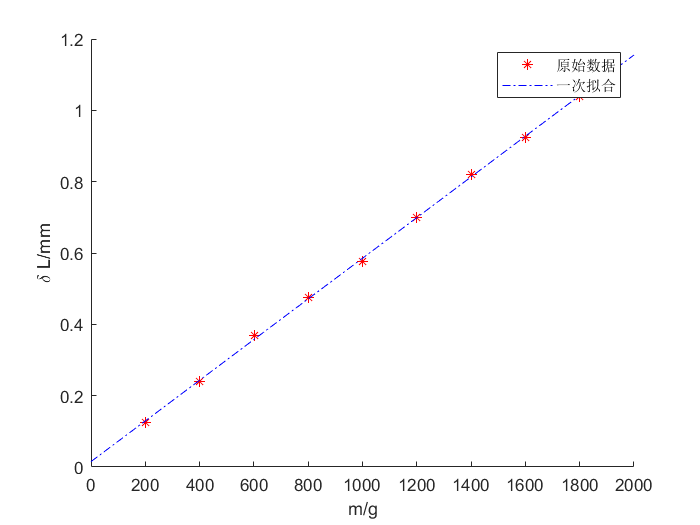
\includegraphics[width=9cm]{huigui.png}
		\caption{最小二乘法线性回归图}
	\end{figure}
由于$k=\dfrac{4gL}{\pi d^2 E}$,则$E=\dfrac{4gL}{\pi d^2 k}\approx 1.675\times10^{11}(Pa)$.又根据公式$\sigma_k=\dfrac{\sigma_{\delta L}}{\sqrt{\sum_{i=1}^{9}(m_i-\bar m)^2}}$,则有$\sigma_{k1}=\dfrac{0.05/\sqrt{3}}{1.5489\times 10^3}=1.86\times10^{-5}$,$\sigma_{k2}=k\sqrt{\dfrac{1/R^2-1}{7}}=4.31\times 10^{-6}$,最终$\sigma_k=\sqrt{\sigma_{k1}^2+\sigma_{k2}^2}=1.91\times10^{-5}$.
由于$E=\dfrac{4gL}{\pi d^2 k}$,则根据方和根合成公式得,
$$
\sigma_E=\sqrt{(\frac{\partial E}{\partial L})^2\sigma_L^2+(\frac{\partial E}{\partial d})^2\sigma_d^2+(\frac{\partial E}{\partial k})^2\sigma_k^2}
$$
\par
最后带入数据算得$\sigma_E=6.1066\times10^{9}(Pa)$,则$E=(1.675\pm0.061)\times 10^{11} Pa$.与逐差法所得的$\sigma_E$相比较,最小二乘法算出来的$\sigma_E$更小一点,显得更为精确.

\subsection*{【选做实验:梁的弯曲测定杨氏模量】}
矩形梁的长度为$l=23.20cm$、厚度为$h=1.359mm$、宽度为$a=10.55mm$.由于测量时间的有限,则在测量梁的厚度和宽度时并没有多次测量,因此暂不考虑它们的随机误差,只考虑仪器造成的误差.则$l=(23.20\pm0.06)cm,h=(1.359\pm0.002)mm,a=(10.55\pm0.03)mm$.\par
测量梁材料的杨氏模量公式为$E=\dfrac{mgl^3}{4\lambda ah^3}$,下面是测量数据:\par
\begin{table}[htbp]
\centering
\caption{测量梁受外力拉伸后的伸展变化数据表}
\scalebox{1.25}{
\begin{tabular}{ccccc}
\toprule
$i$&$m_i/g$&$r_i/mm$&$r_i^{\prime}/mm$&$\bar r_i/mm$ \\
\hline
0&0.00&34.611&33.568&34.0895 \\
1&200.48&33.569&32.348&32.9585 \\
2&400.53&32.400&31.121&31.7605 \\
3&600.44&31.212&29.959&30.5855 \\
4&800.52&30.041&28.779&29.4100 \\
5&1000.81&28.822&27.685&28.2535\\
6&1200.35&27.261&26.646&26.9535 \\
\bottomrule
\end{tabular}}
\end{table}
现在为了逐项逐差,因此去掉第一组数据,再逐三项逐差.\par
则$\bar E=\dfrac{(1.9778+1.9539+1.9086)\times10^{11}}{3}=1.947\times10^{11}(Pa)$.
\subsection*{【分析与讨论】}
开始情况下,$r$比正常量大的原因是金属丝有弯曲;而$r$比正常量小的原因是金属丝有扭曲或者接触处有摩擦.我的数据为前者这种情况,可能是金属丝使用过多导致有些弯曲没法消除.




\end{document}